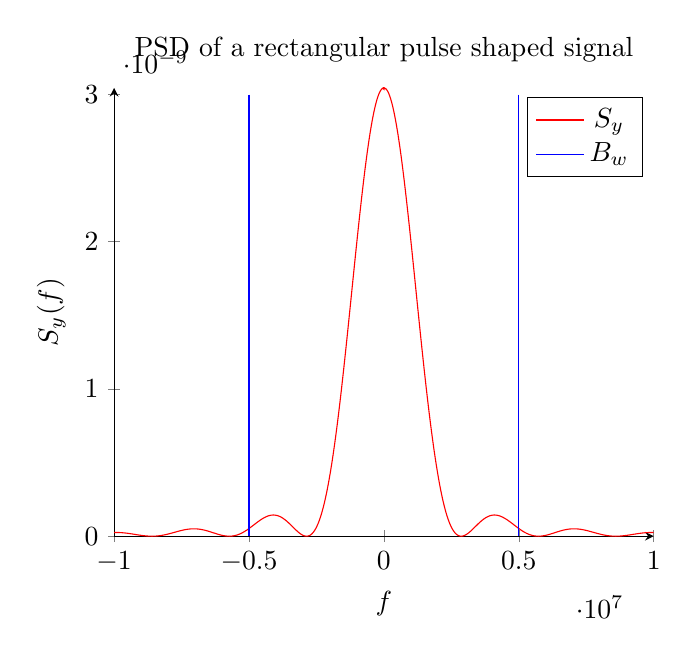
\begin{tikzpicture}
    \begin{axis}[
        axis lines = left,
        xlabel = $f$,
        ylabel = {$S_y(f)$},
        title = PSD of a rectangular pulse shaped signal,
    ]
    \addplot [
        domain=-10000000:10000000, 
        samples=2000, 
        color=red,
    ]
    {2500000*0.000002^2*((sin(x*pi*0.00002))/(x*pi*0.00002))^2};
    \addlegendentry{$S_y$}

    \addplot [
        color=blue,
    ]
    coordinates {(5000000, 0.000000003) (5000000, 0)};
    \addplot [
        color=blue,
    ]
    coordinates {(-5000000, 0.000000003) (-5000000, 0)};
    \addlegendentry{$B_w$}
    
    \end{axis}
\end{tikzpicture}
